\documentclass[12pt]{article}
\usepackage{graphicx}

\title{Práctica 3: Memorias Asociativas Dinámicas}
\author{Manuel González González}
\begin{document}
\maketitle
\section*{Ejercicio 1}
\subsection*{a)}
Los patrones de entrada han de ser ortolineales para que no se solapen los resultados, por eso usamos los patrones (A,AS), (B,BS), (C,CS) y (D,DS).
\subsection*{b)}
Para que no se reconozca correctamente, los patrones deben ser no ortonormales, por lo cual es suficiente con cambiar los patrones de entrada por unos que cumplan dicha condición.\\
Devuelve salidas incorrectas debido a que no es capaz de memorizar los patrones no ortogonales, pues se superponen en la matriz de pesos.

\section*{Ejercicio 2}
\subsection*{a)}
Se estabiliza en el patrón memorizado.
\subsection*{b)}
Se estabiliza en el inverso del patrón memorizado. Esto se debe a que más de la mitad del patrón difiere del aprendido.
\subsection*{c)}
No existe ninguna entrada que difiera del patrón memorizado o de su opuesto, ya que solo se ha memorizado un patrón. La salida solo puede ser una de las dos anteriores.
\subsection*{d)} 
Depende de la cantidad de elementos que coincidan o no con la entrada original (patrón memorizado). En caso de que coincida más de la mitad, la salida es el patrón original; en caso contrario, el resultado es el opuesto. 

\subsection*{e)}
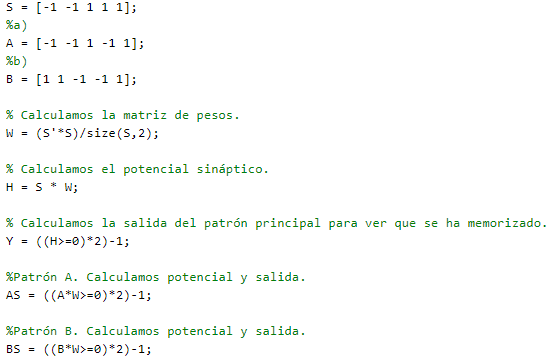
\includegraphics[scale=1]{AsociadorNoLineal.png} 

\section*{Ejercicio 3}

\subsection*{a)}
Se han usado 63 unidades de proceso (9*7).
\subsection*{b)}
Comete errores en la C, D y E. Esto se debe a que los patrones se parecen entre sí y no difieren lo suficiente como para que los memorice de forma independiente.
\subsection*{c)}
Le sale un punto en mitad que intenta representar la segunda horizontal de la E, debido a que la representación de ambos patrones es similar.

\subsection*{d)}
En este caso no comete error. Esto se debe a que la cantidad de patrones a memorizar es menor; y a que los patrones entre sí son lo suficientemente distintos como para que no haya distorsiones.
\end{document}
